\documentclass[a4j]{ujarticle}
\usepackage[dvipdfmx]{graphicx}
\usepackage{url}
\usepackage{bbding}
\usepackage{lscape}
\usepackage[subrefformat=parens]{subcaption}
\usepackage{bm}
\usepackage{amsmath}

\title{ミーティング資料}
\author{安達智哉\\to-adachi@ist.osaka-u.ac.jp}
\date{2019年4月10日}

\begin{document}
\maketitle



\section{Server Disaggregation}
\subsection{Server Disaggregationに関する先行研究}
Intel CorporationのWhite Paper \cite{DisaggregatedServersDriveDataCenterEfficiencyandInnovation}では、Disaggregated Serverに基づくインテル®ラックスケールアーキテクチャを示している。
このアーキテクチャでは、マザーボード上でCPU / DRAMモジュールとNIC /ドライブモジュールを分離している。
この手法より、CPUとメモリを他のコンポーネントを交換することなく、交換することが可能であり、コンピューティングおよびストレージのパフォーマンスや容量を手頃な価格で向上させることができる。
交換作業は簡単であり、従来のように何時間もかかることはない。
4本のネジを外してCPU / DRAMモジュールをスライドさせ、新しいCPU / DRAMモジュールを取り付けることで交換作業は完了すると述べている。
サーバの構成を図\ref{intel-server}に示す。
また、交換作業の工程と所要時間を図\ref{intel-refresh}に示す。

\begin{figure}[htbp]
  \centering
  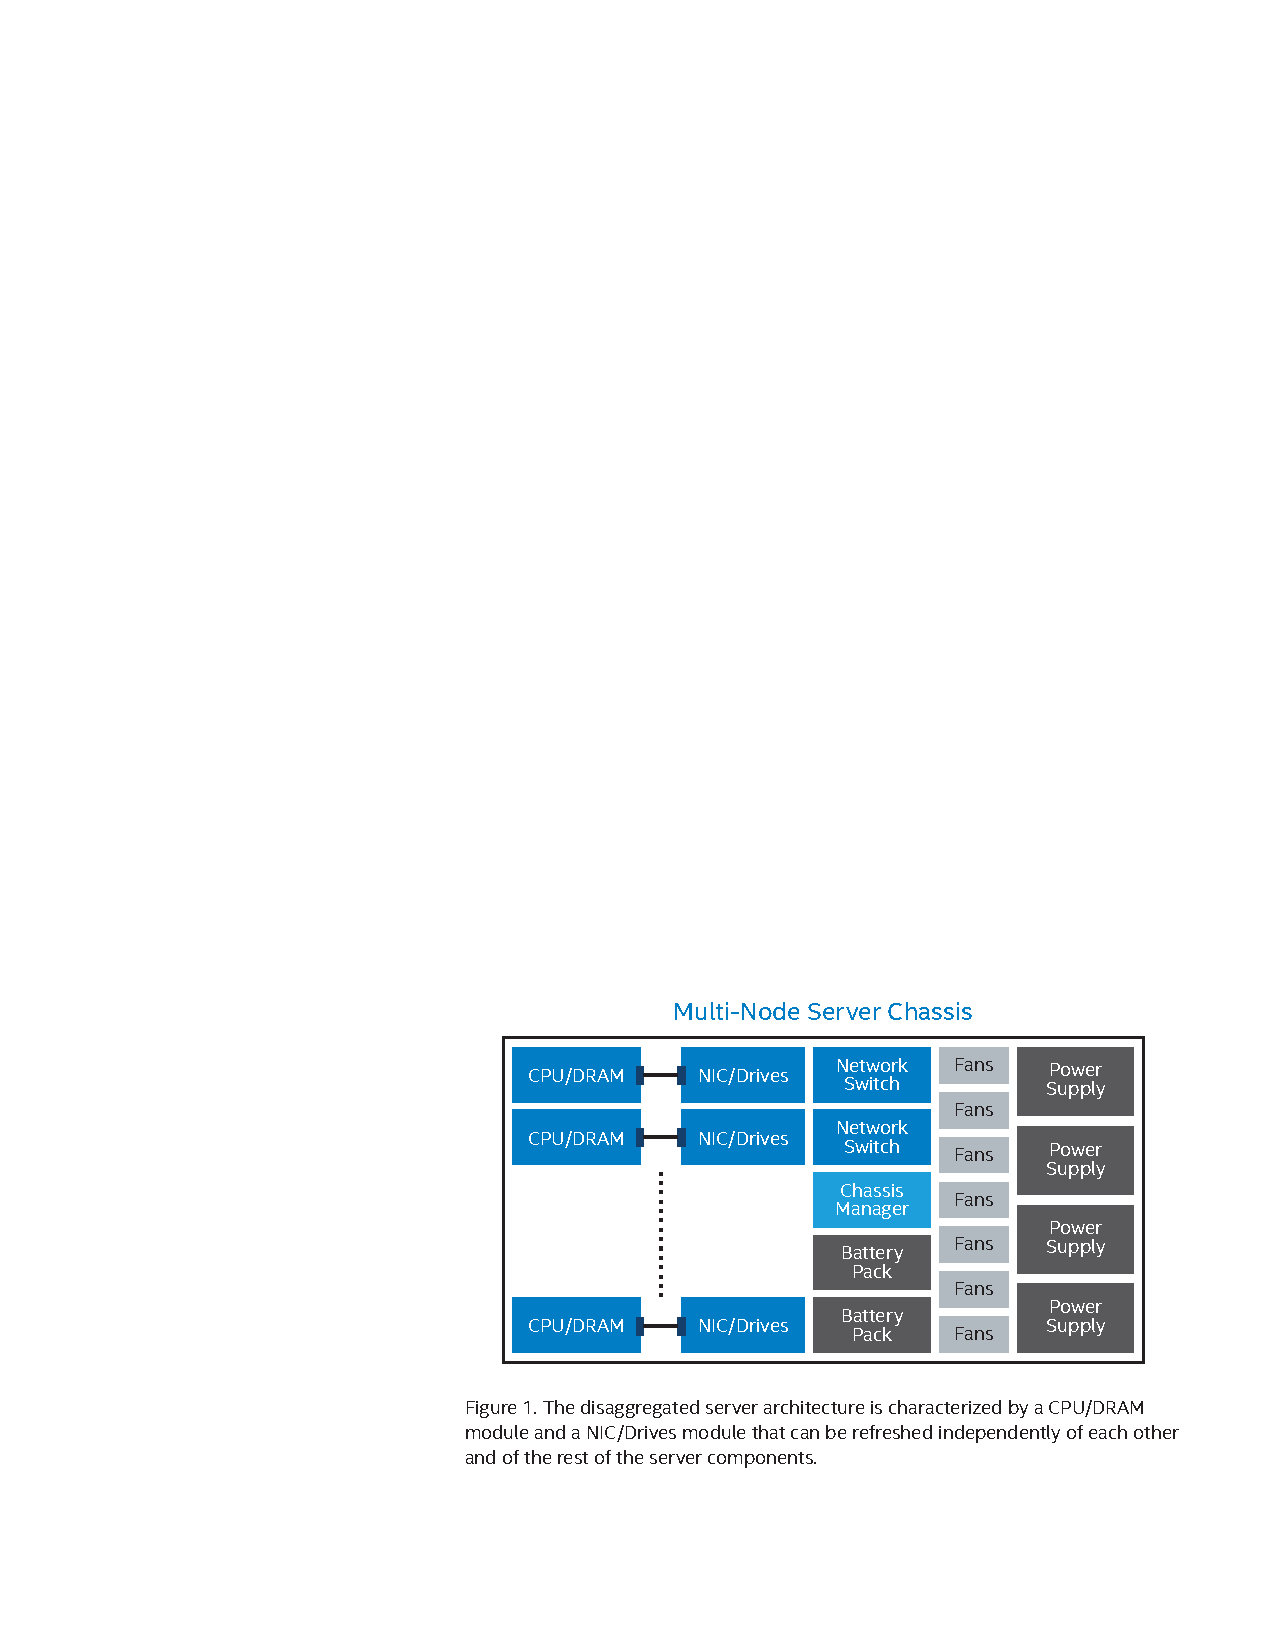
\includegraphics[width=1.0\hsize]{intel-server.pdf}
  \caption{サーバ構成}
  \label{intel-server}
\end{figure}

\begin{figure}[htbp]
  \centering
  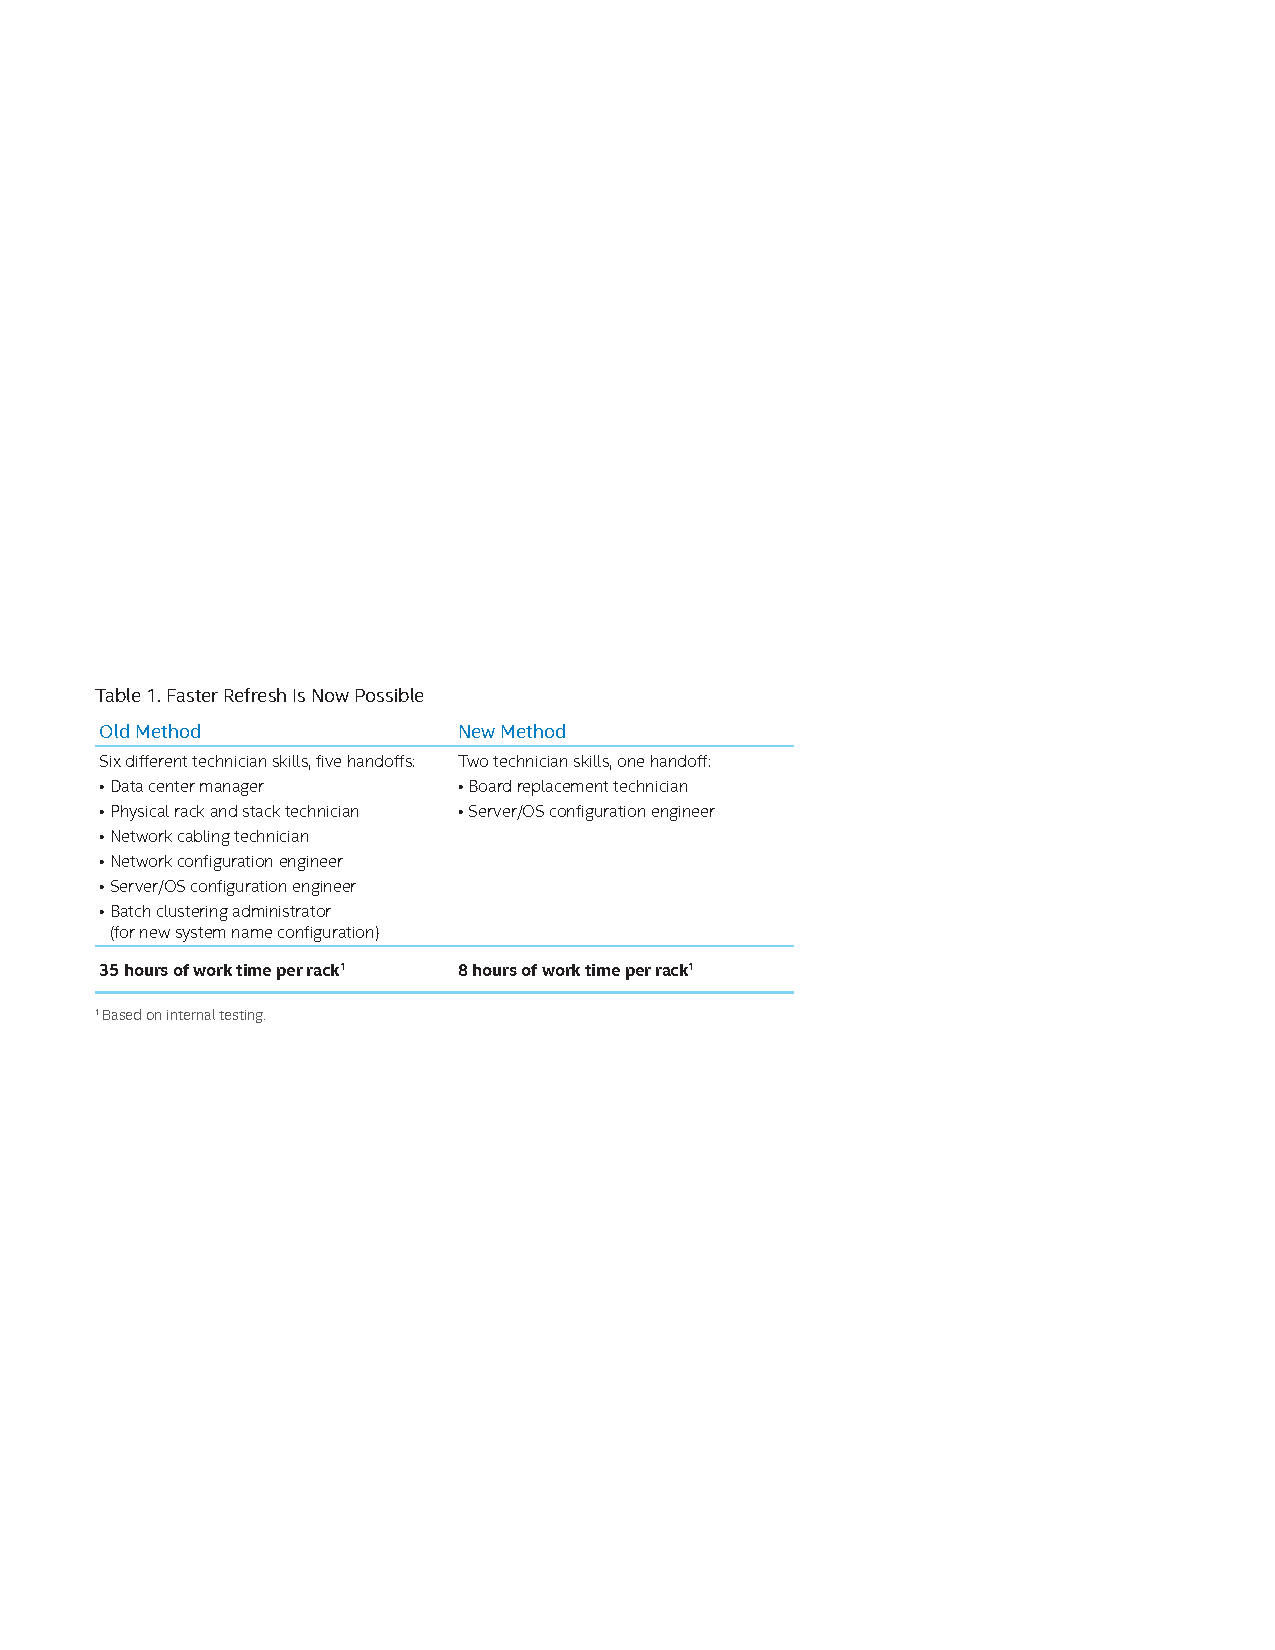
\includegraphics[width=1.0\hsize]{intel-refresh.pdf}
  \caption{コンポーネントの交換工程}
  \label{intel-refresh}
\end{figure}

また、文献\cite{IntelsDisaggregatedServerRack}、\cite{EnhancedBackoffTimerSolutionforGTPCOverloadControl}では、CPUとメモリの分離も前提としたDisaggregated Server アーキテクチャについて述べている。
課題は、CPUとメモリ間のネットワークの構成である。
一つは、新しいメモリアーキテクチャを必要とすることである。
CPUとメモリを分離することにより、両者の物理的な距離が増大する。
これに対応するためは、両者を結ぶネットワーク帯域幅の大きな飛躍を必要とする。
現在Intelでは、光ファイバーケーブルの束を必要とし、CPUとメモリを接続することを想定している。しかし、それをサポートするためには全く新しいクラスのスイッチアーキテクチャを設計しなければならないと考えられる。
Intelが想定する将来の分離型ラックは、以下の要素から構成されると述べている。
\begin{itemize}
  \item 複数個のプロセッサトレイ
  \item 複数個のシステムメモリトレイ
  \item SSDもしくはHDDからなる多数のストレージトレイ
  \item 上記のトレイをすべて結び付けるファブリックネットワーク
\end{itemize}


文献\cite{UnderstandingRackScaleDisaggregatedStorage}では、サーバとストレージをラックスケールで分離し、制御の時間スケールが与える影響について調査している。この文献では、最も時間スケールの細かい制御として、IO処理毎にストレージ構成を変化させるモデルを想定している。この場合、ストレージの再割り当てに伴うオーバーヘッドが大きくなると述べている。
一方、複数のIO処理を実行する間、ストレージ構成を変化させないモデルを想定した場合、IOごとにストレージ構成を変化させるモデルと比較して、大幅にオーバヘッドが軽減されると述べている。また、ストレージ構成を変化させる頻度は、数日から数時間になると述べている。
図\ref{disaggregated_time}に制御のタイムスケールの細かさとその特徴をまとめた表を示す。また、図\ref{disaggregated_overhead}にIOごとにストレージ構成を変化させるモデルにおいて発生するオーバヘッドを示す。
\begin{figure}[htbp]
  \centering
  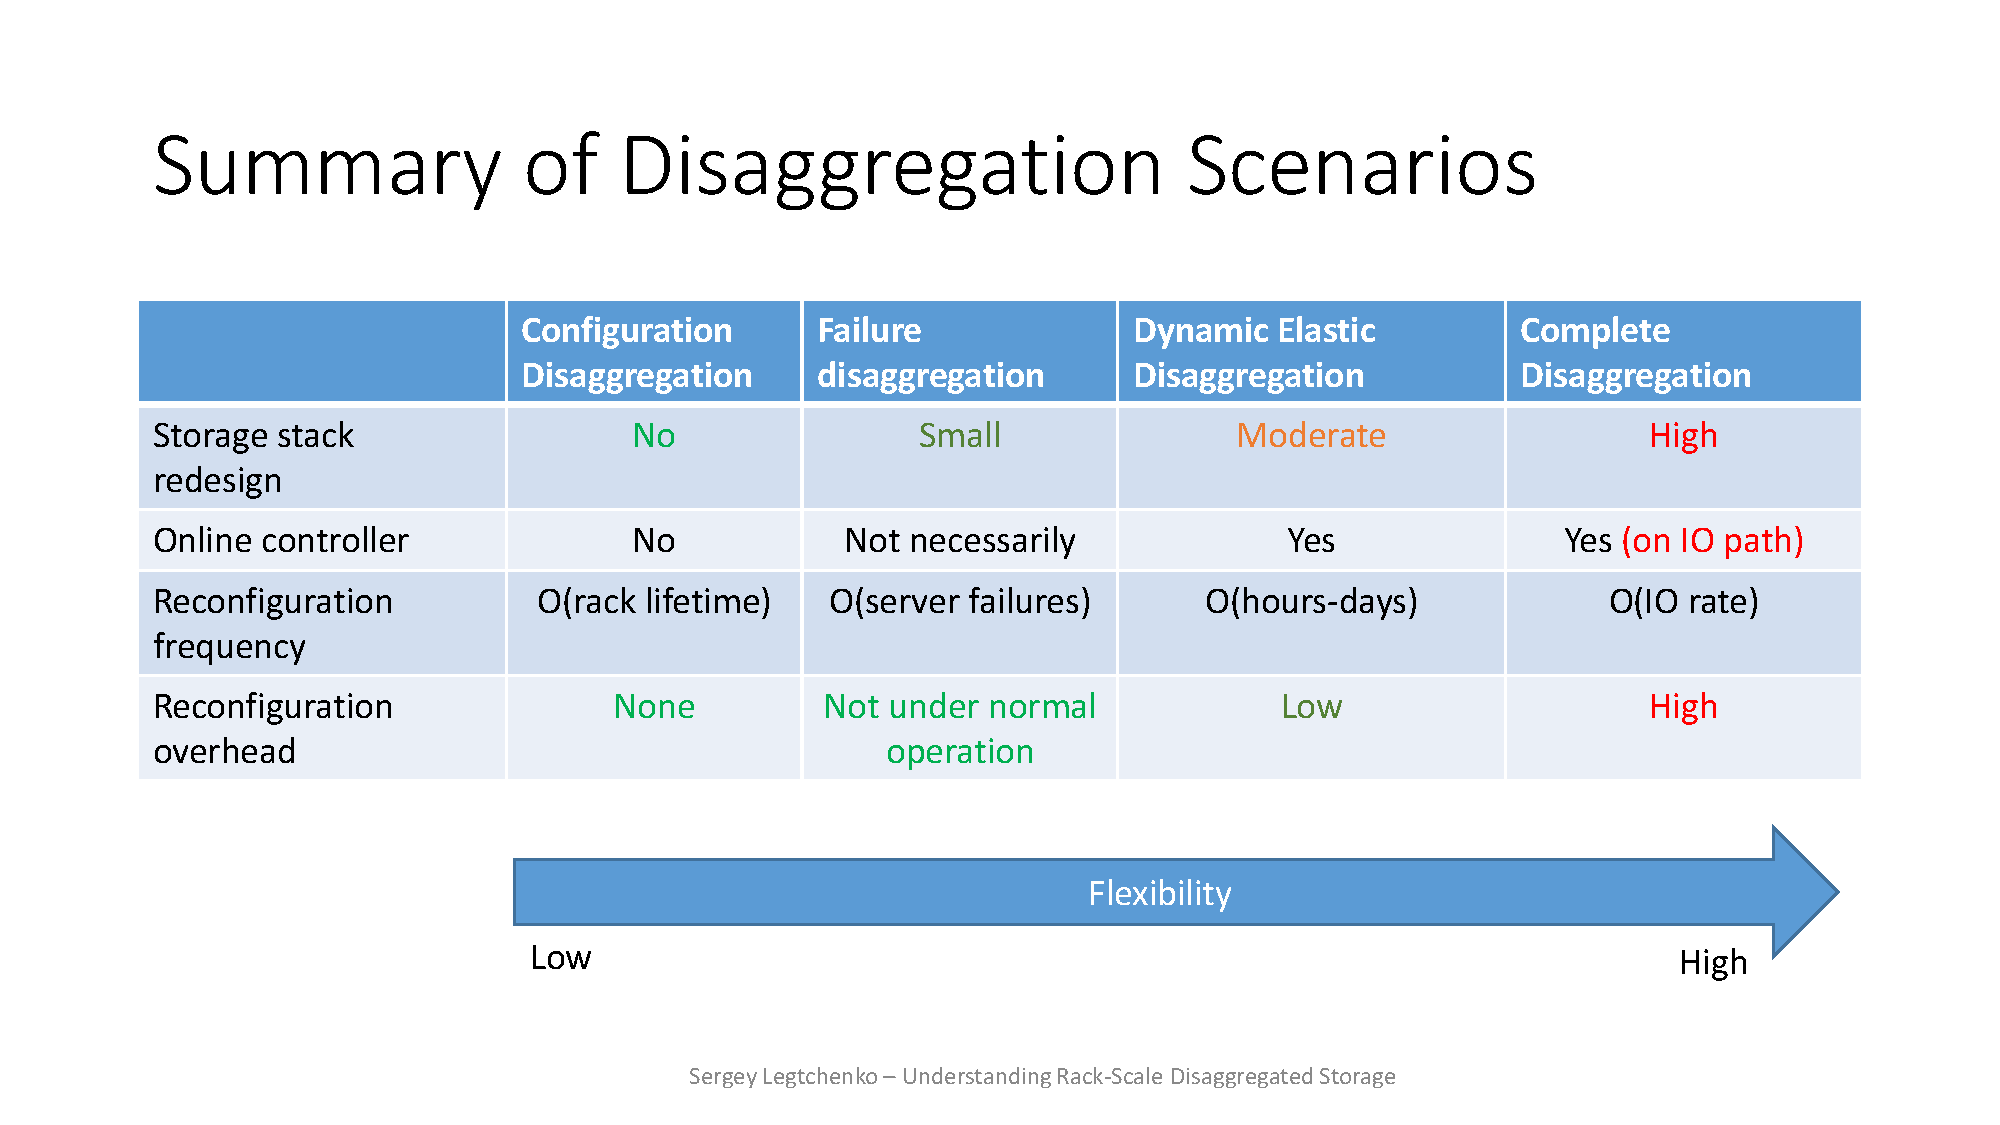
\includegraphics[width=1.0\hsize]{disaggregated_time.pdf}
  \caption{ストレージ構成の制御のタイムスケールの細かさとその特徴}
  \label{disaggregated_time}
\end{figure}
\begin{figure}[htbp]
  \centering
  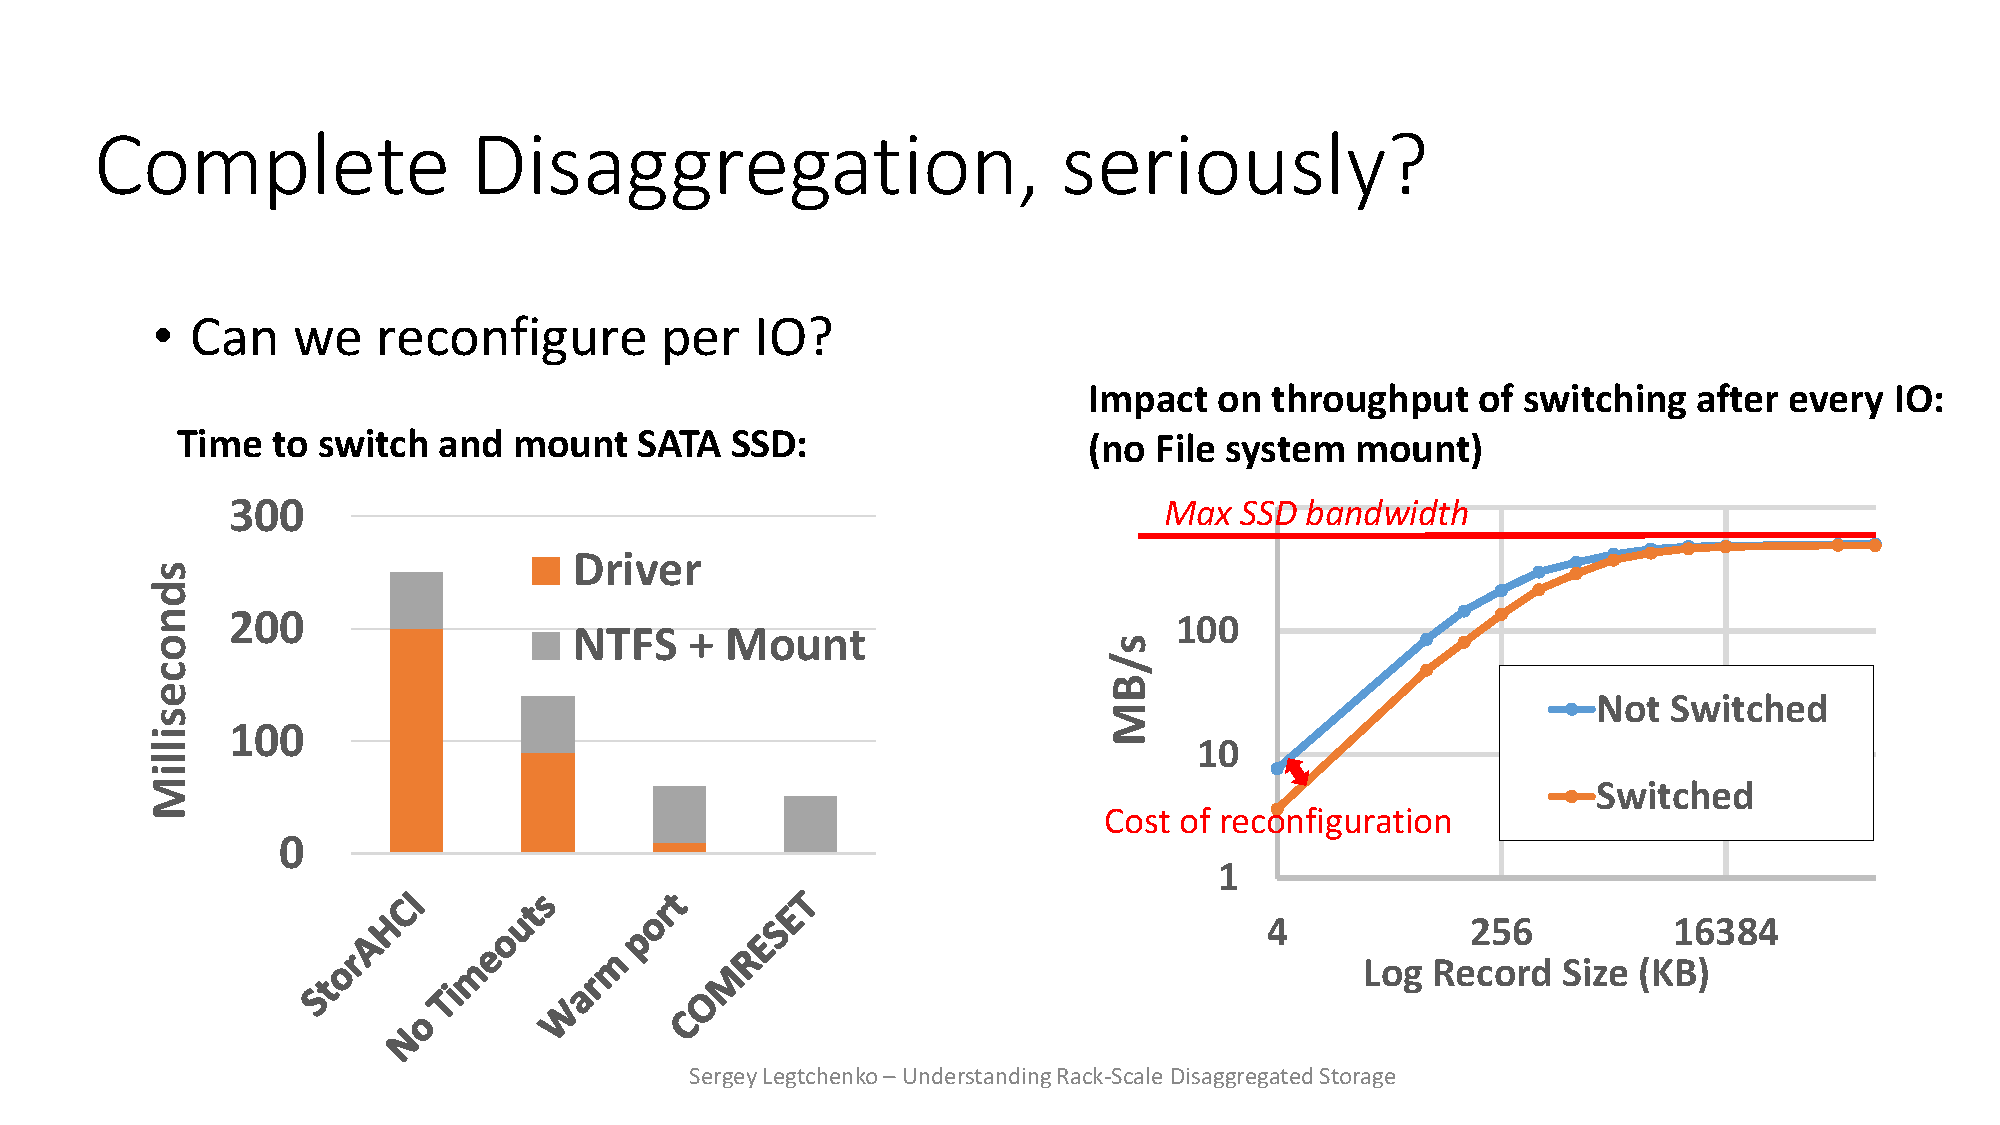
\includegraphics[width=1.0\hsize]{disaggregated_overhead.pdf}
  \caption{細かいタイムスケールでのストレージ構成制御を行った場合のオーバーヘッド}
  \label{disaggregated_overhead}
\end{figure}

\clearpage
文献\cite{ComposableArchitectureforRackScaleBigDataComputing}では、リソースを分離した際の主な課題として、メモリ、SSD/HDD、GPU/FPGAなどのリモートリソースプールにアクセスする際にインターコネクトとスイッチで発生する待ち時間を挙げている。
その理由は、リモートリソースプールのアクセスレイテンシが本来のアクセスレイテンシと比較して大幅に増大すると、プロセッサ、ハイパーバイザ、OS、またはアプリケーションレベルでスレッドの並列処理が利用されない限り、パフォーマンスが大幅に低下する可能性があると述べている。
また、リソース分離の規模として、ラック単位、PoD単位、データセンタ単位の3種類を想定している。
それぞれのモデルを図\ref{rack}及び図\ref{PoD_Data}に示す。

今日ローカルに接続されたメモリにアクセスするための帯域幅と待ち時間は、それぞれ920 Gb /秒と75 nsである。
PCIeスイッチ(第3世代)は150 ns程度の遅延を発生させ、トップオブラックIPスイッチおよびInfinibandスイッチの遅延は最大800 nsである。
そのためこの文献では、ラックを超えてメモリリソースを分離するためには、シリコンフォトニクスと光回路スイッチ(OCS)が唯一の選択肢であると述べている\cite{TheEmergingOpticalDataCenter,ADemonstrationofUltralowlatencyDataCenterOpticalCircuitSwitching,DeliveringScaleOutDataCenterNetworkingwithOpticsWhyandHow}。
そして、そのようなネットワークの構成は、従来のものと比べてはるかに高いコストであると述べている\cite{DisaggregatedandOpticallyInterconnectedMemoryWhenwillitbecosteffective}。

またこの文献では、以下に示すようなさまざまなインターコネクトおよびスイッチテクノロジのポート間レイテンシを仮定した上で、GPU/FPGA、SSD/HDDのリソースに関しては、低遅延のTORスイッチ、PCIeスイッチ、またはInfiniBandスイッチを用いることで簡単にリソース分離が可能であるとも結論付けている。
\begin{itemize}
  \item Arista製などの低レイテンシTORスイッチ$(380〜1000 ns)$\cite{AristaNetworksCloudNetworkingPortfolio}
  \item Arista製などの低レイテンシ spine-leaf スイッチ$(2〜10\mu s)$\cite{AristaNetworksCloudNetworkingPortfolio}
  \item Mellanox製のInfiniBandスイッチ$(700 ns)$
  \item Calient製の光回線スイッチ$(< 30 ns)$\cite{CalientS320Datasheet}
  \item PCIeスイッチなどH3プラットフォームで作成されたもの$(〜150 ns)$
  \item ラック、PoD、およびデータセンターの往復伝搬遅延$5 ns/m$
  \item ラック内:平均伝搬距離$3m(15ns)$
  \item Intra PoD:平均伝搬距離$50m (250ns)$
  \item データセンター内:平均伝搬距離$200m (1\mu s)$
\end{itemize}
上記の結果をまとめたものを図\ref{network_data}に示す。

\begin{figure}[htbp]
  \centering
  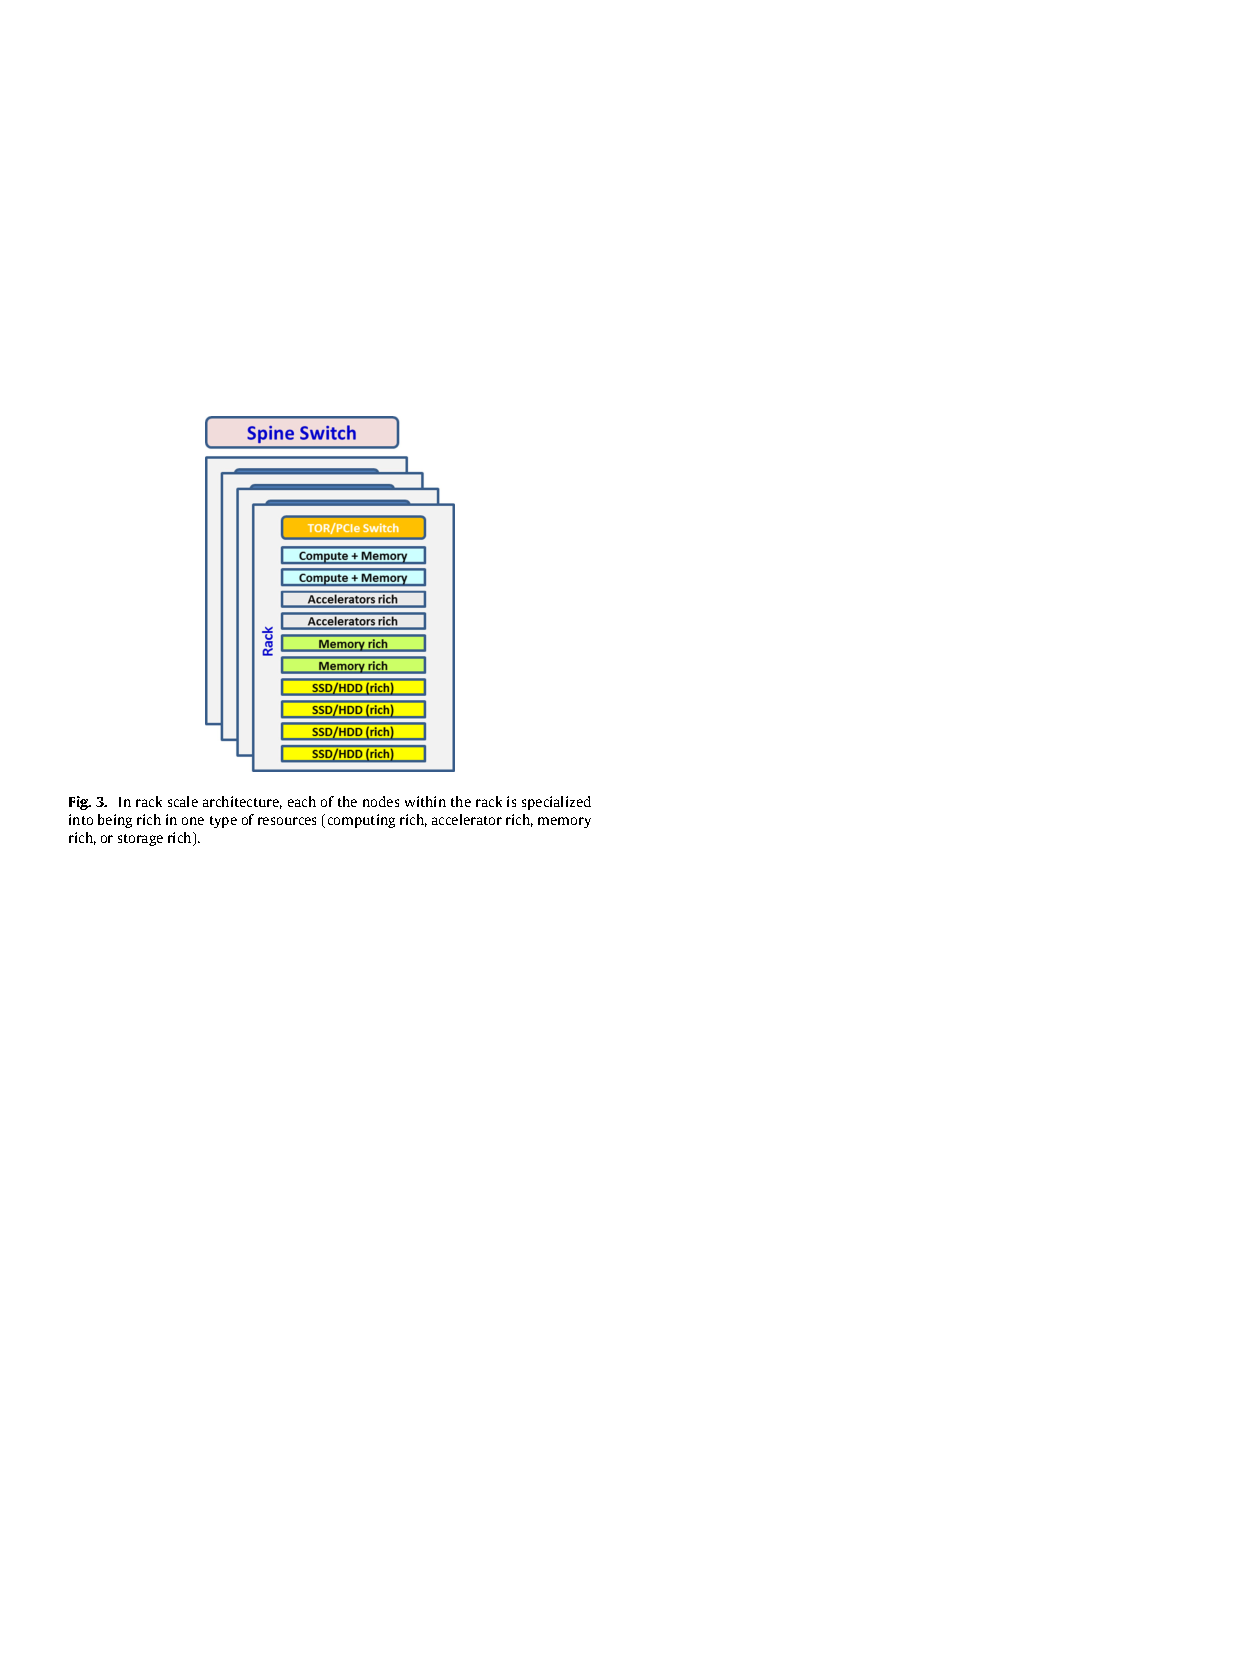
\includegraphics[width=0.7\hsize]{rack.pdf}
  \caption{ラックスケールでのリソース分離モデル}
  \label{rack}
\end{figure}
\begin{figure}[htbp]
  \centering
  \includegraphics[width=0.7\hsize]{PoD_Data.pdf}
  \caption{PoD及びデータセンタ規模でのリソース分離モデル}
  \label{PoD_Data}
\end{figure}

\begin{figure}[htbp]
  \centering
  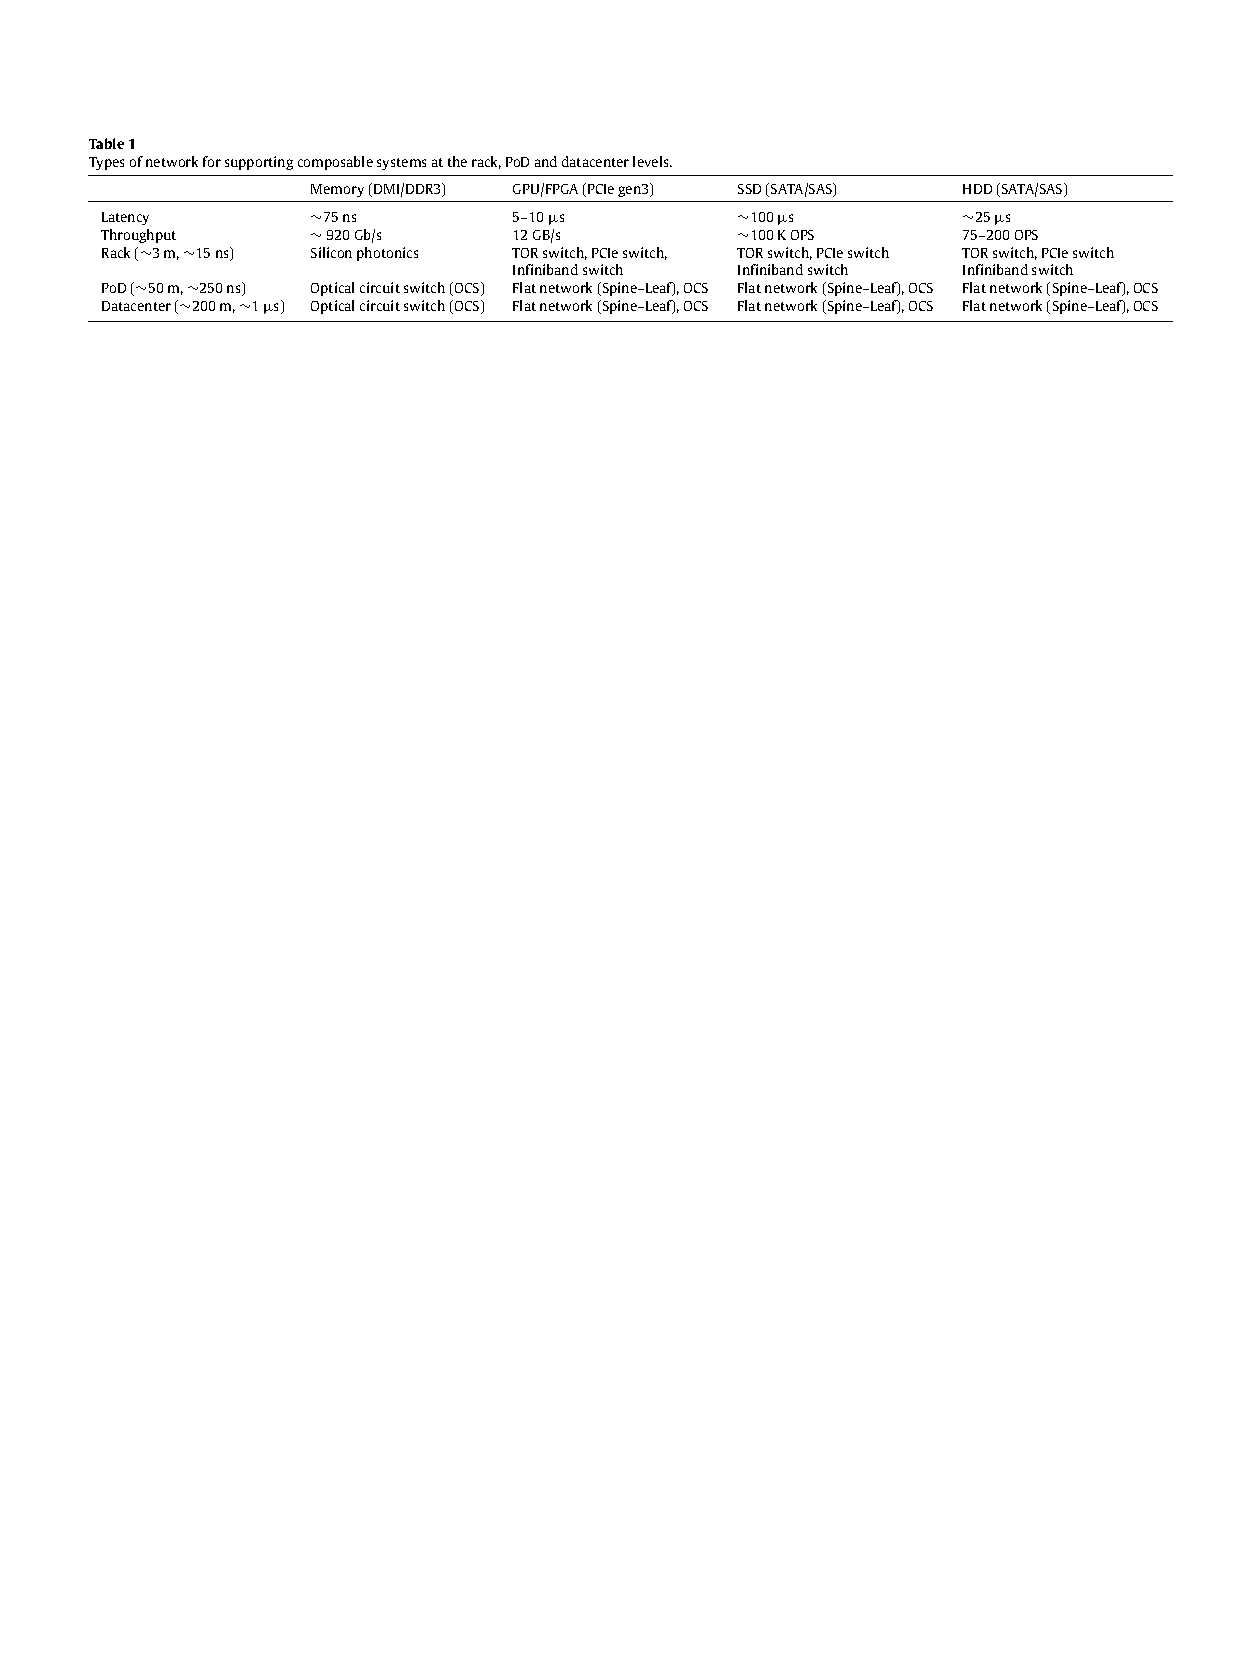
\includegraphics[width=1.0\hsize]{network_data.pdf}
  \caption{各リモートリソースプールにアクセスする際の遅延制約とそれを満たすためのネットワーク構成}
  \label{network_data}
\end{figure}

\clearpage
\subsection{Server Disaggregationと私の研究との関係}
現在のモバイルネットワークでは、EPCノードにおけるCPUとメモリのリソース消費の予測が難しような状況や変動が大きいような状況においても、どちらかがボトルネックにならずに、効率的にリソースを活用するアーキテクチャを考えることは重要である。
% このような背景から、EPCノードにおけるCPUとメモリのリソース消費の予測が難しような状況や変動が大きいような状況においても、どちらかがボトルネックにならずに、効率的にリソースを活用するアーキテクチャを考えることは重要である。
実際、CPUとメモリのリソースを効率よく活用する研究は、データセンタなどの分野では行われている。
文献\cite{TechnoEconomicFrameworkforCloudInfrastructureACostStudyofResourceDisaggregation}では、server disaggregation の考えをデータセンタに適用し、CPUやメモリなどのリソースをモジュール化し、需要に合わせて自由に組み替えることを可能にすることにより、リソースの効率的な利用が可能であることを示している。
しかし、server disaggregation にはいくつかの課題がある。
まず、CPUとメモリのリソースを分離するためには、大きなコストがかかる点が挙げられる。
文献\cite{IntelsDisaggregatedServerRack}、\cite{EnhancedBackoffTimerSolutionforGTPCOverloadControl}では、CPUとメモリを分離するためには、両者を結ぶための新しい高帯域ネットワークが必要になると述べている。また、両者の物理的な距離が増加することによって発生する遅延も考慮する必要があるため、新たなメモリアーキテクチャの構築が必要であると述べている。
文献\cite{DisaggregatedandOpticallyInterconnectedMemoryWhenwillitbecosteffective}では、メモリを分離するためには、低遅延かつ高帯域のネットワーク接続が必要となるが、それを実装するためにコストは従来と比較して大幅に増加すると述べている。
実際、文献\cite{DisaggregatedServersDriveDataCenterEfficiencyandInnovation}では、Disaggregated Serverに基づくインテルのラックスケールアーキテクチャを示しているが、このモデルでもCPUとメモリの分離はできていない。
課題の2つ目として、短いタイムスケールでの制御が難しいという問題が挙げられる。
例えば、ストレージをモジュール化してサーバと分離する手法について述べられている文献\cite{UnderstandingRackScaleDisaggregatedStorage}では、時間スケールの細かいストレージ制御を行った場合、ストレージの再割り当て処理に伴うオーバーヘッドが大きくなると述べている。
また、頻繁にリソース構成を変化させることは、コスト面や消費電力の面でも不利である(注:まだ根拠はない)。

このように、server disaggregation を用いたリソース制御では、リソース制御に伴うオーバーヘッドの発生が避けては通れない課題となると予想される。
特に、モバイルネットワークのように、突発的なトラヒックの増加が発生し、数分以下のオーダでリソース量の制御を行う必要があるネットワークにおいては細かいタイムスケールでの効率的なリソース制御が求められる。

そこで、本研究ではモバイルネットワークに特化した、柔軟かつ効率的な、EPCノードにおけるCPUとメモリ間の負荷のオフロード方法を考案する。
具体的には、ネットワークの負荷に合わせて、UEの状態を制御することにより、メモリおよびCPUに与える負荷のバランスを変化させる。
UEの状態の制御は、UEが最後にデータを送信したあと、Connected Inactive状態からIdle状態に遷移するまでの時間を設定することで実現する。
この方法により、CPUが過負荷である場合は、UEが最後にデータを送信したあと、Connected Inactive状態からIdle状態に遷移するまでの時間を長く設定することにより、メモリの負荷を増加させる代わりにCPUの負荷を削減することが可能である。
またその逆に、メモリが過負荷である場合は、この時間を短く設定することにより、CPUの負荷を増加させる代わりにメモリの負荷を削減できる。
この時間の再設定処理は、数分単位のオーダーで可能でありかつ、それに伴い発生するオーバーヘッドは、server disaggregation と比較して僅かである(注:提案手法のオーバーヘッドの大小に関する記述は、今後の研究結果によって修正します)。
また、既存のシグナリングアーキテクチャに変更を加えることが可能であれば、秒単位の時間スケールでの制御も可能であると考えられる。

しかし、提案手法には限界もある。
それは、対応可能なリソース需要に制限があることである。
なぜなら、提案手法では、限られたCPUおよびメモリのリソースを効率的に利用することは可能であるが、双方のリソースが過負荷になるようなリソース需要には対応できないからである。
特に長期的かつ大規模なリソース需要の変化に対しては、server disaggregation を用いたリソース制御の方が適している。
また、提案手法を用いなかった場合には常時Connected Inactive 状態であったUEが、提案手法を用いることによりIdle状態へと遷移する可能性があるため、データを送受信にかかる遅延時間が増加するなど、QoSの低下が発生する可能性がある。
しかし、電気メータや気温計のようなリアルタイム性を必要としないIoT端末であれば、これらのQoSの低下は無視できると考えられる。

そのため、提案手法とserver disaggregationやスケールアウト/スケールインを組み合わせることにより、より効果のあるリソース管理が可能であると考えられる。
例えば、長期的かつ大規模なリソース制御はserver disaggregationを用いて行う一方で、server disaggregation で対応できないような短いタイムスケールでのリソース制御は提案手法を用いて行う。
もしくは、リソース需要の大きな変動に対してはスケールアウト/スケールインを用いて対応した上で、細かなリソース需要の変化に対しては提案手法を用いて対応する。
上述ように、server disaggregationやスケールアウト/スケールインと提案手法組み合わせ、双方のデメリットを補うことで、モバイルネットワークのリソース制御をより良く実現できると考えられる。


\section{UEの状態遷移に伴う、シグナリングの発生数の調査}
\subsection{Idle状態からConnected状態への遷移}
文献\cite{3gpp.23.720}に示されている、コネクション確立に伴うシグナリング図を図\ref{Legacy_connection_setup}に示す。
この図を見ることによって、UEがIdle状態からConnected状態に遷移する際に各ノードで処理する(送受信する)シグナリングの数は以下の様に求めることができる。
\begin{itemize}
  \item UE      :9
  \item eNodeB  :12
  \item MME     :5
  \item SGW     :2
\end{itemize}
\begin{figure}[htbp]
  \centering
  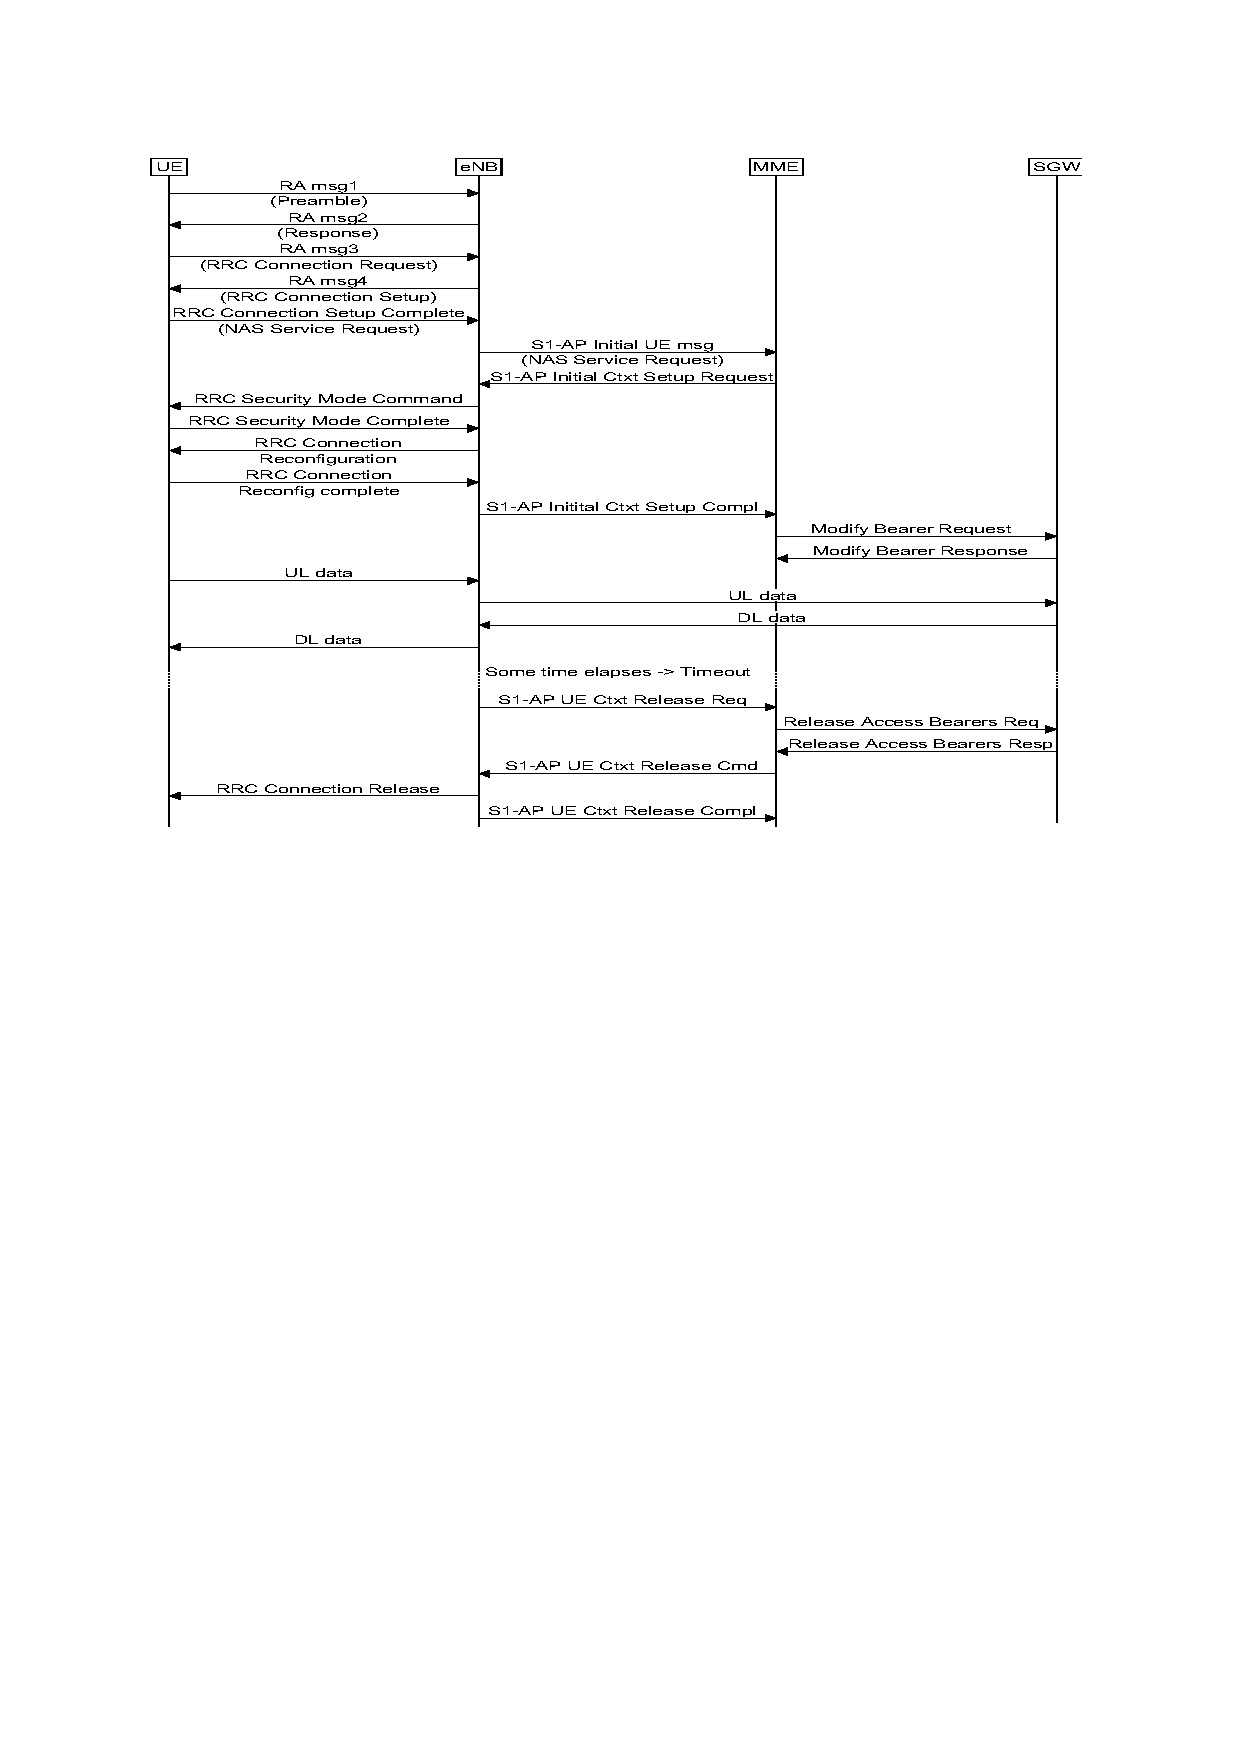
\includegraphics[width=0.9\hsize]{Legacy_connection_setup.pdf}
  \caption{Legacy connection setup}
  \label{Legacy_connection_setup}
\end{figure}
\clearpage
\subsection{Connected Inactive状態からConnected状態への遷移}
\label{sec:cennectedinactive-connected}
文献\cite{ANovelStateModelfor5GRadioAccessNetworks}では、RRC Connected Inactive 状態からConnected状態へ遷移する際のシグナリング図を示していた。そのシグナリング図を図\ref{Signaling_for_the_RRC_CONNECTED_INACTIVE_to_RRC_CONNECTED_transition_for_the_novel_state_model}に示す。
図\ref{Signaling_for_the_RRC_CONNECTED_INACTIVE_to_RRC_CONNECTED_transition_for_the_novel_state_model}を見ると、UE-RAN間のシグナリングが5回発生していることがわかる。
また、コアネットワーク側にはシグナリングは発生していないこともわかる。
UEがConnected Inactive状態からConnected状態に遷移する際に各ノードで処理するシグナリングの数は以下の様になる。
\begin{itemize}
  \item UE      :5
  \item eNodeB  :5
  \item MME     :0
  \item SGW     :0
\end{itemize}\begin{figure}[htbp]
  \centering
  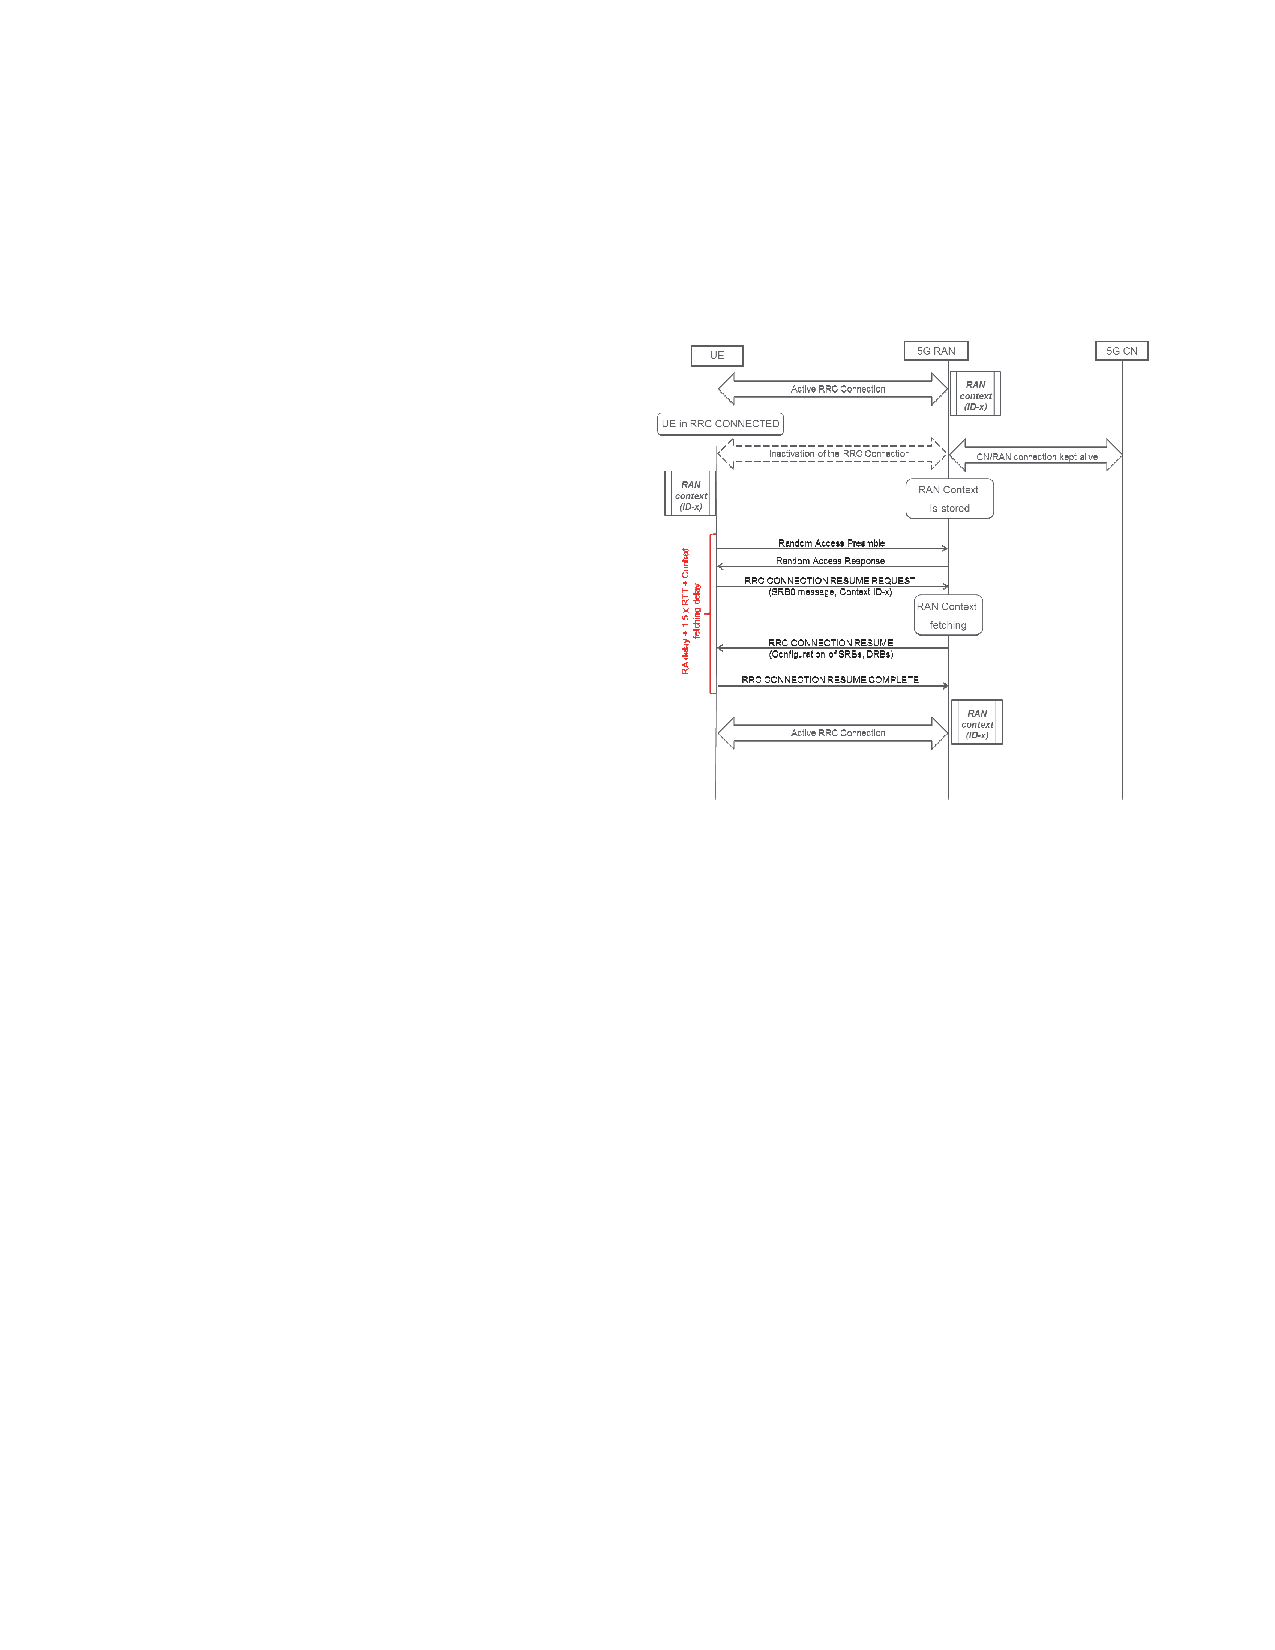
\includegraphics[width=0.9\hsize]{Signaling_for_the_RRC_CONNECTED_INACTIVE_to_RRC_CONNECTED_transition_for_the_novel_state_model.pdf}
  \caption{Signaling for the RRC CONNECTED INACTIVE to RRC CONNECTED transition for the novel state model}
  \label{Signaling_for_the_RRC_CONNECTED_INACTIVE_to_RRC_CONNECTED_transition_for_the_novel_state_model}
\end{figure}
\clearpage
\subsection{Connected状態からIdle状態への遷移}
\label{sec:connected-idle}
Connected状態からIdle状態へ遷移する際に発生するシグナリングに関しては、図\ref{Legacy_connection_setup}を見ることで確認できる。
具体的には、図\ref{Legacy_connection_setup}のS1-AP UE Ctxt Relese Req 以降のシグナリングが、Connected状態からIdle状態へ遷移する際に発生するシグナリングに該当する。
このシグナリングでは、eNodeBおよびMMEの持っているUEのコンテキストおよび、MMEとSGWのベアラ、RRCコネクションの解放を行っている。
UEがConnected状態からIdle状態に遷移する際に各ノードで処理するシグナリングの数は以下の様になる。
\begin{itemize}
  \item UE      :1
  \item eNodeB  :4
  \item MME     :5
  \item SGW     :2
\end{itemize}
\subsection{Connected状態からConnected Inactive状態への遷移}
\label{sec:connected-connectedinactive}
Connected状態からConnected Inactive状態へ遷移する際に発生するシグナリングに関しては、図\ref{Legacy_connection_setup}、図\ref{Signaling_for_the_RRC_CONNECTED_INACTIVE_to_RRC_CONNECTED_transition_for_the_novel_state_model}および第\ref{sec:cennectedinactive-connected}節、第\ref{sec:connected-idle}節を参考にすることにより推定可能である。

まず、図\ref{Signaling_for_the_RRC_CONNECTED_INACTIVE_to_RRC_CONNECTED_transition_for_the_novel_state_model}および第\ref{sec:cennectedinactive-connected}節より、Connected Inactive 状態からConnected状態へ遷移する際には、UE-eNodeB間においてRRCコネクションを確立するためのシグナリングのみが発生し、コアノード側にはシグナリングが発生しないことがわかる。
このことから、Connected状態からConnected Inactive状態への遷移する場合は、RRCコネクションを解放するためのシグナリングが発生する一方でコアノード側にはシグナリングは発生しない可能性が高いと予想できる。

RRCコネクションを解放する際に発生するシグナリングの数は、図\ref{Legacy_connection_setup}および第\ref{sec:connected-idle}節を見ることにより確認できる。

このことから、Connected状態からConnected Inactive状態への遷移するに各ノードで処理するシグナリングの数は以下の様になる。
\begin{itemize}
  \item UE      :1
  \item eNodeB  :1
  \item MME     :0
  \item SGW     :0
\end{itemize}
\subsection{Connected Inactive状態からIdle状態への遷移}
Connected Inactive状態からIdle状態へ遷移する際に発生するシグナリングに関しては、第\ref{sec:connected-idle}節および第\ref{sec:connected-connectedinactive}節で求めたシグナリング数を比較することにより推定可能である。
第\ref{sec:connected-idle}節では、Connected状態からIdle状態に遷移する際にはUEのコンテキストおよびMMEとSGWのベアラ、RRCコネクションの解放を行うと述べた。
また、第\ref{sec:connected-connectedinactive}節では、Connected状態からConnected Inactive状態への遷移する際には、RRCコネクションを解放すると述べた。
以上の知見から、Connected状態からIdle状態に遷移する際のシグナリングから、RRCコネクションの解放に関するシグナリングを除いたものが、Connected Inactive状態からIdle状態への遷移する際のシグナリングと推定できる。
その際に各ノードで処理するシグナリングの数は以下の様になる。
\begin{itemize}
  \item UE      :0
  \item eNodeB  :3
  \item MME     :5
  \item SGW     :2
\end{itemize}
\subsection{Connected Inactive状態における、状態遷移を伴わないデータ送信}
文献\cite{RRCStateHandlingfor5G}では、小さなデータ量であれば、Connected Inactive状態からConnected状態へ遷移することなく、データ送信が可能であると述べている。
まず、UE-eNodeB間においてRA preambleおよびRA responseシグナリングを実行する。
その後、UEからeNodeBに対してRRC Active Messageを送信するが、それに対してデータをピギーバックする。
最後に、eNodeBからUEに対して、RRC Inactivate Messageを送信してシグナリングは処理は終了である。
その際に各ノードで処理するシグナリングの数は以下の様になる。
\begin{itemize}
  \item UE      :4
  \item eNodeB  :4
  \item MME     :0
  \item SGW     :0
\end{itemize}


%
%
% \subsection{先行研究~1}
% RRC Connected Inactive及びRRC Suspendedに関して述べられている、文献\cite{RRCStateHandlingfor5G}では、UEがConnected状態へ遷移する際に発生するシグナリング数は表\ref{table:signalings}ようになると述べられている。
% RRC Suspended 状態ではUEのコンテキストの一部がUE及びネットワークに保持されているため、シグナリング数が減少している。
% また、RRC Connected Inactive 状態では、RAN-コアネットワーク間の接続がkeep aliveとなっているため、RAN-コアネットワーク間のシグナリングは発生せず、UE-RAN間のシグナリングのみが発生する。
% \begin{table}[htbp]
%   \centering
%   \caption{Signaling Overhead}
%   \label{table:signalings}
%   \begin{tabular}{ccccc}
%     \hline
%     遷移元                  & 遷移先              & \multicolumn{3}{c}{シグナリング数} \\
%                             &                     & 無線      & S1     & S11     \\ \hline \hline
%     Idle                    & Connected           & 9         & 3      & 2       \\
%     RRC Suspended           & Connected           & 5         & 2      & 2       \\
%     RRC Connected Inactive  & Connected           & 4         & 0      & 0       \\ \hline
%   \end{tabular}
% \end{table}
%
% この文献\cite{RRCStateHandlingfor5G}では、IdleとRRC Suspended に関するシグナリング数に対しては、3GPPの仕様書\cite{3gpp.23.720}を根拠として示している。
% 文献\cite{3gpp.23.720}に示されている図を図\ref{Legacy_connection_setup}及び図\ref{Resumption_of_a_previously_suspended_RRC_connection}に示す。
% これらの図を見ることによって、表\ref{table:signalings}に示されているシグナリング数を確認することが可能である。
% また、MMEが処理するべきシグナリング数(MMEが送受信するシグナリング数)は、Idle及びRRC Suspendedそれぞれにおいて5個、4個であることがわかる。
% しかし一方で、RRC Connected Inactive に関するシグナリング数に対しては参考文献を示していなかった。
%
% \begin{figure}[htbp]
%   \centering
%   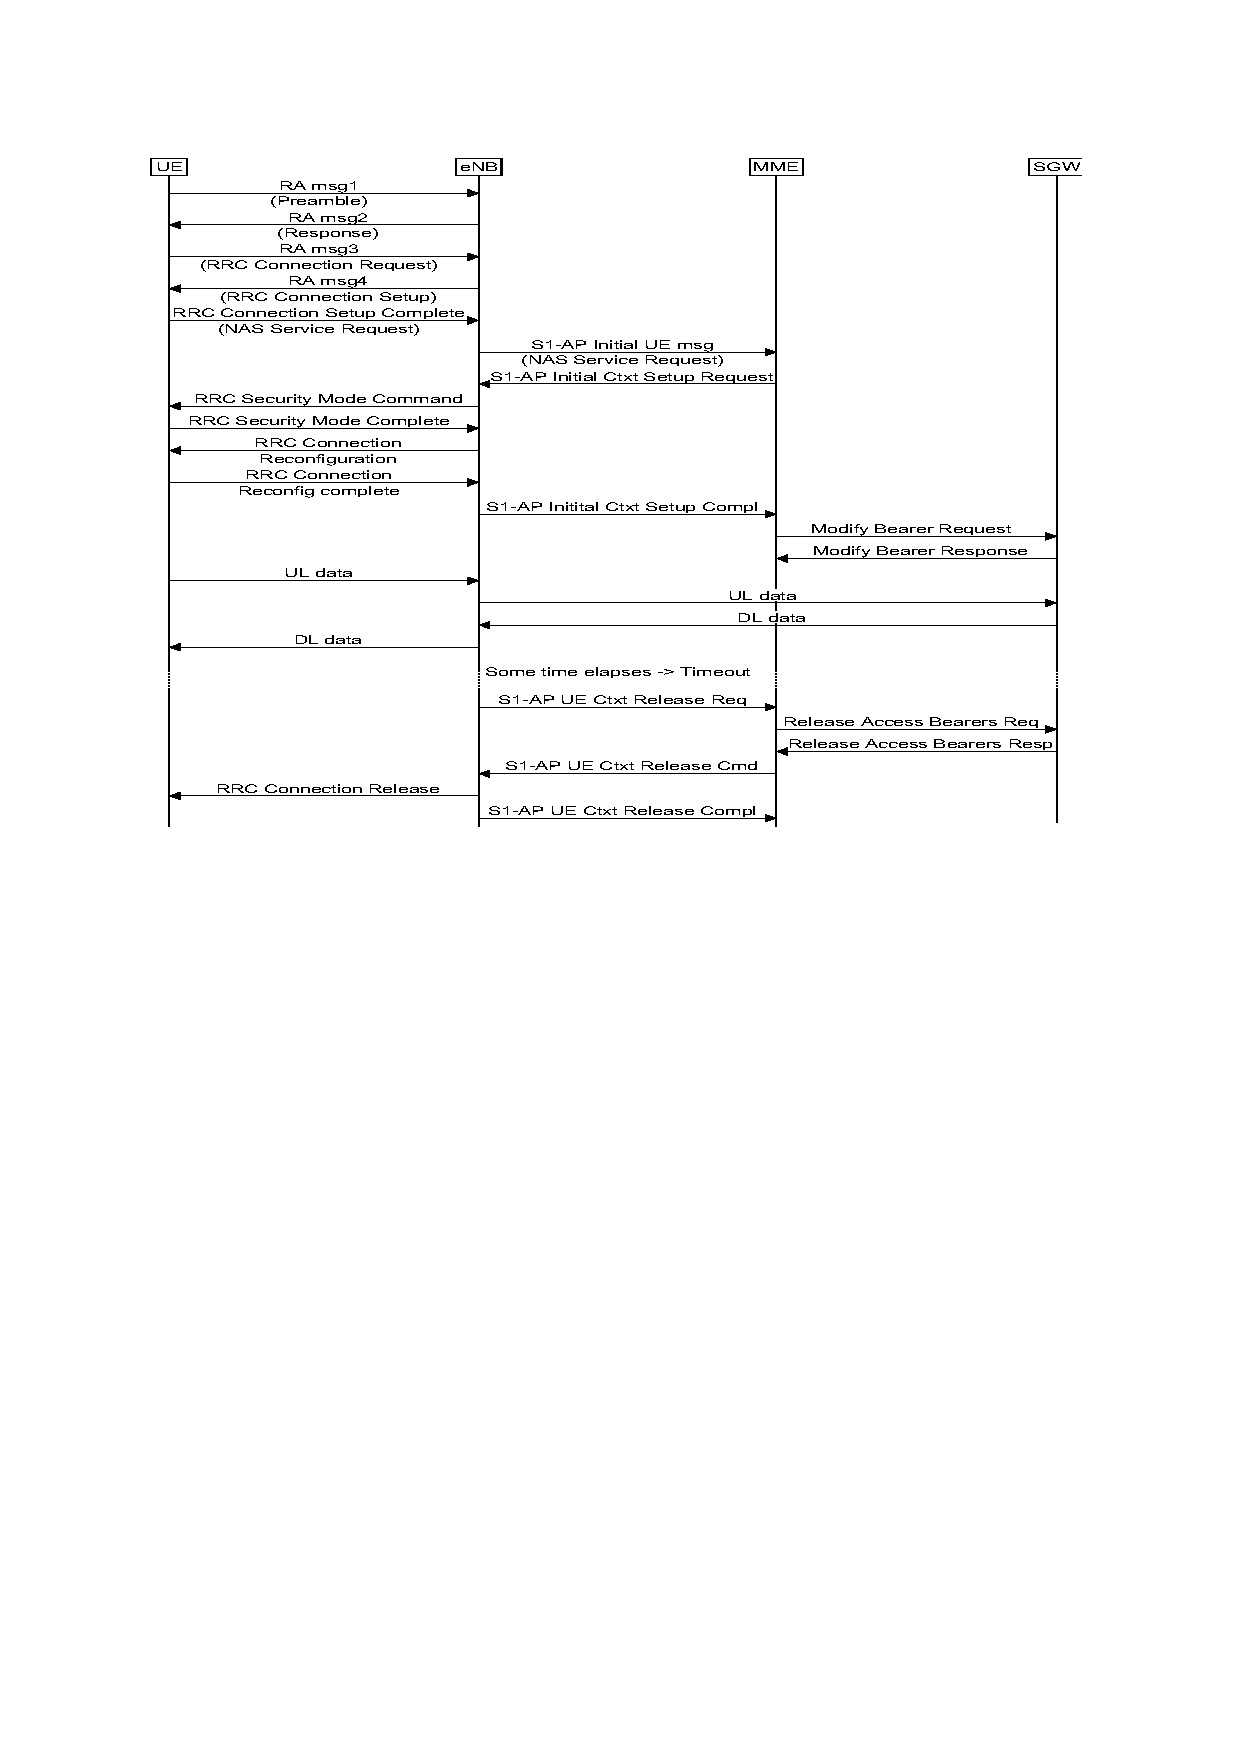
\includegraphics[width=0.9\hsize]{Legacy_connection_setup.pdf}
%   \caption{Legacy connection setup}
%   \label{Legacy_connection_setup}
% \end{figure}
%
% \begin{figure}[htbp]
%   \centering
%   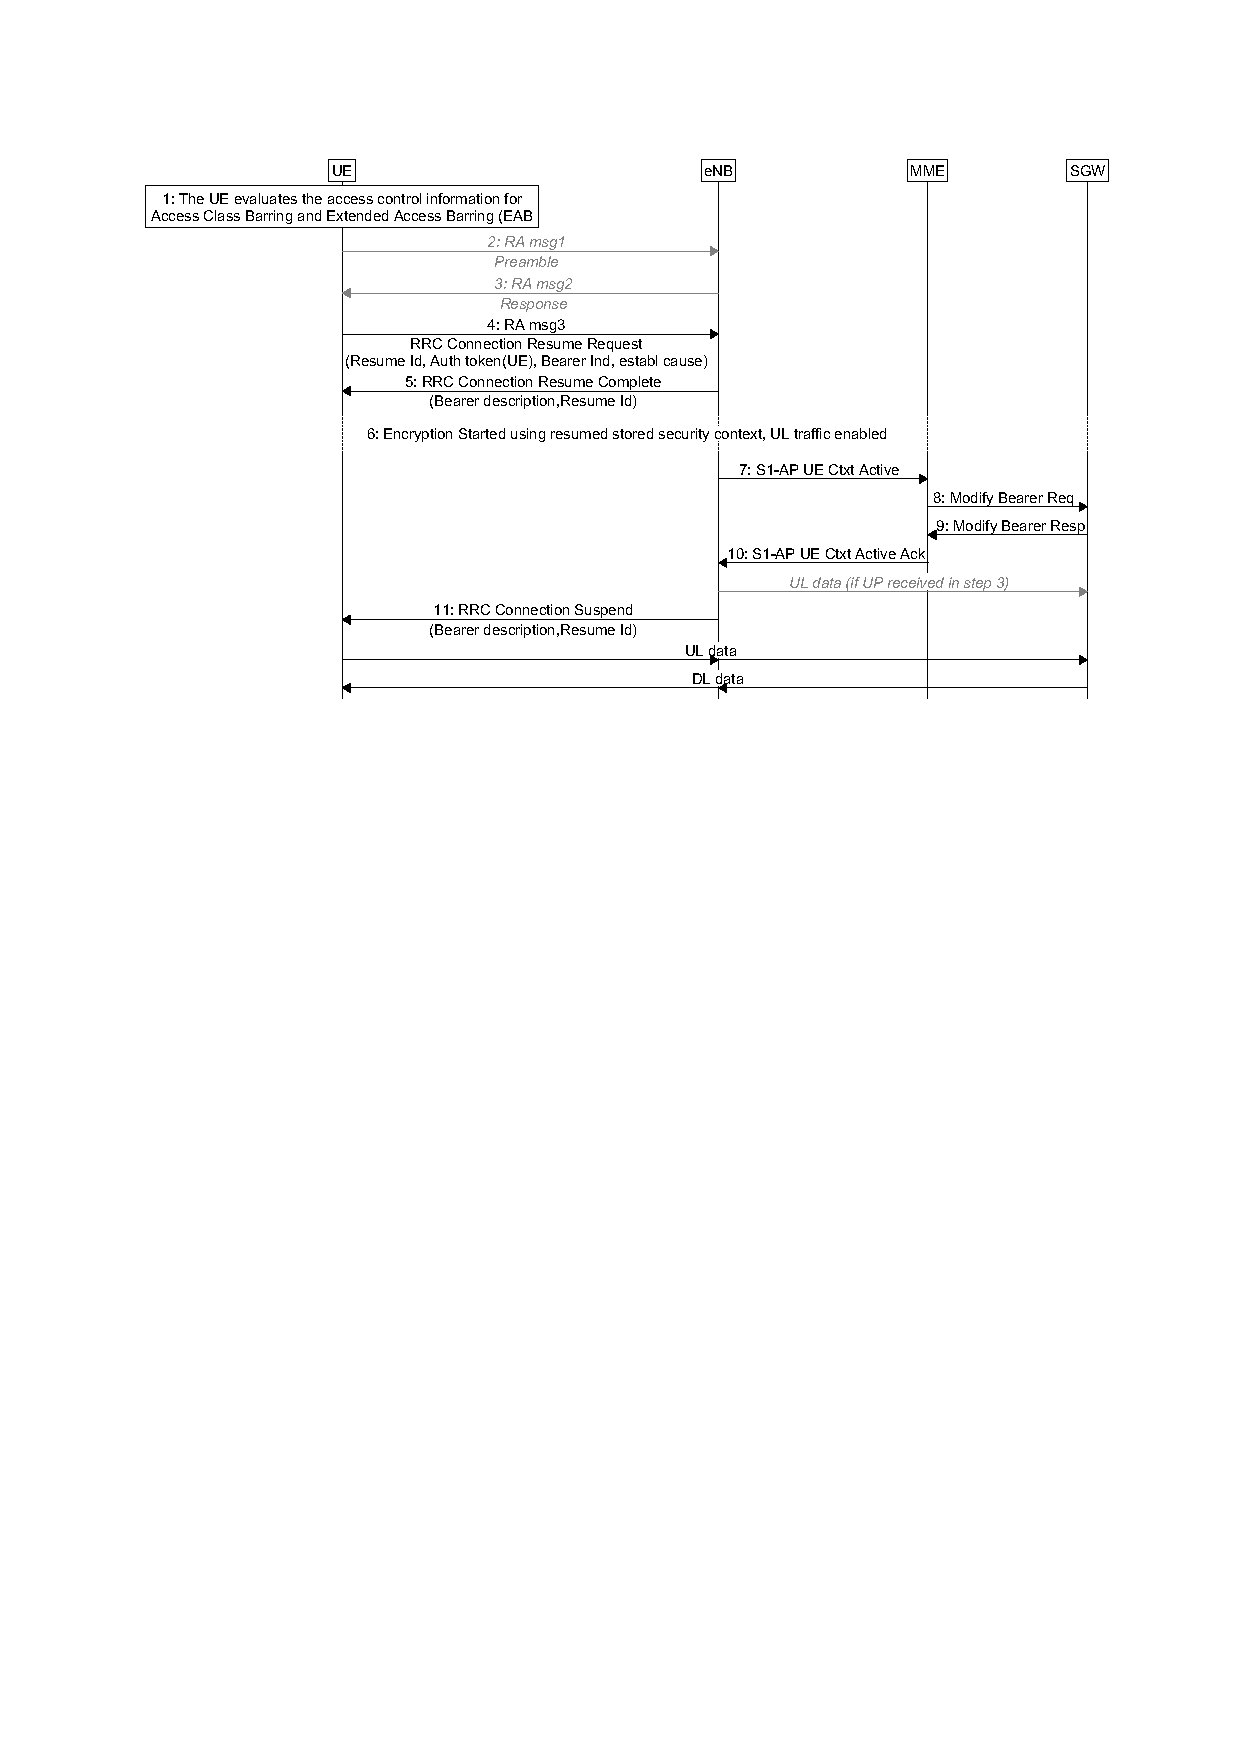
\includegraphics[width=0.9\hsize]{Resumption_of_a_previously_suspended_RRC_connection.pdf}
%   \caption{Resumption of a previously suspended RRC connection}
%   \label{Resumption_of_a_previously_suspended_RRC_connection}
% \end{figure}
%
% \clearpage
% \subsection{先行研究~2}
% 文献\cite{ANovelStateModelfor5GRadioAccessNetworks}では、RRC Connected Inactive 状態からConnected状態へ遷移する際のシグナリング図を示していた。
% そのシグナリング図を図\ref{Signaling_for_the_RRC_CONNECTED_INACTIVE_to_RRC_CONNECTED_transition_for_the_novel_state_model}に示す。
% 図\ref{Signaling_for_the_RRC_CONNECTED_INACTIVE_to_RRC_CONNECTED_transition_for_the_novel_state_model}を見ると、UE-RAN間のシグナリングが5回発生していることがわかる。
% また、コアネットワーク側にはシグナリングは発生していないこともわかる。
%
% \begin{figure}[htbp]
%   \centering
%   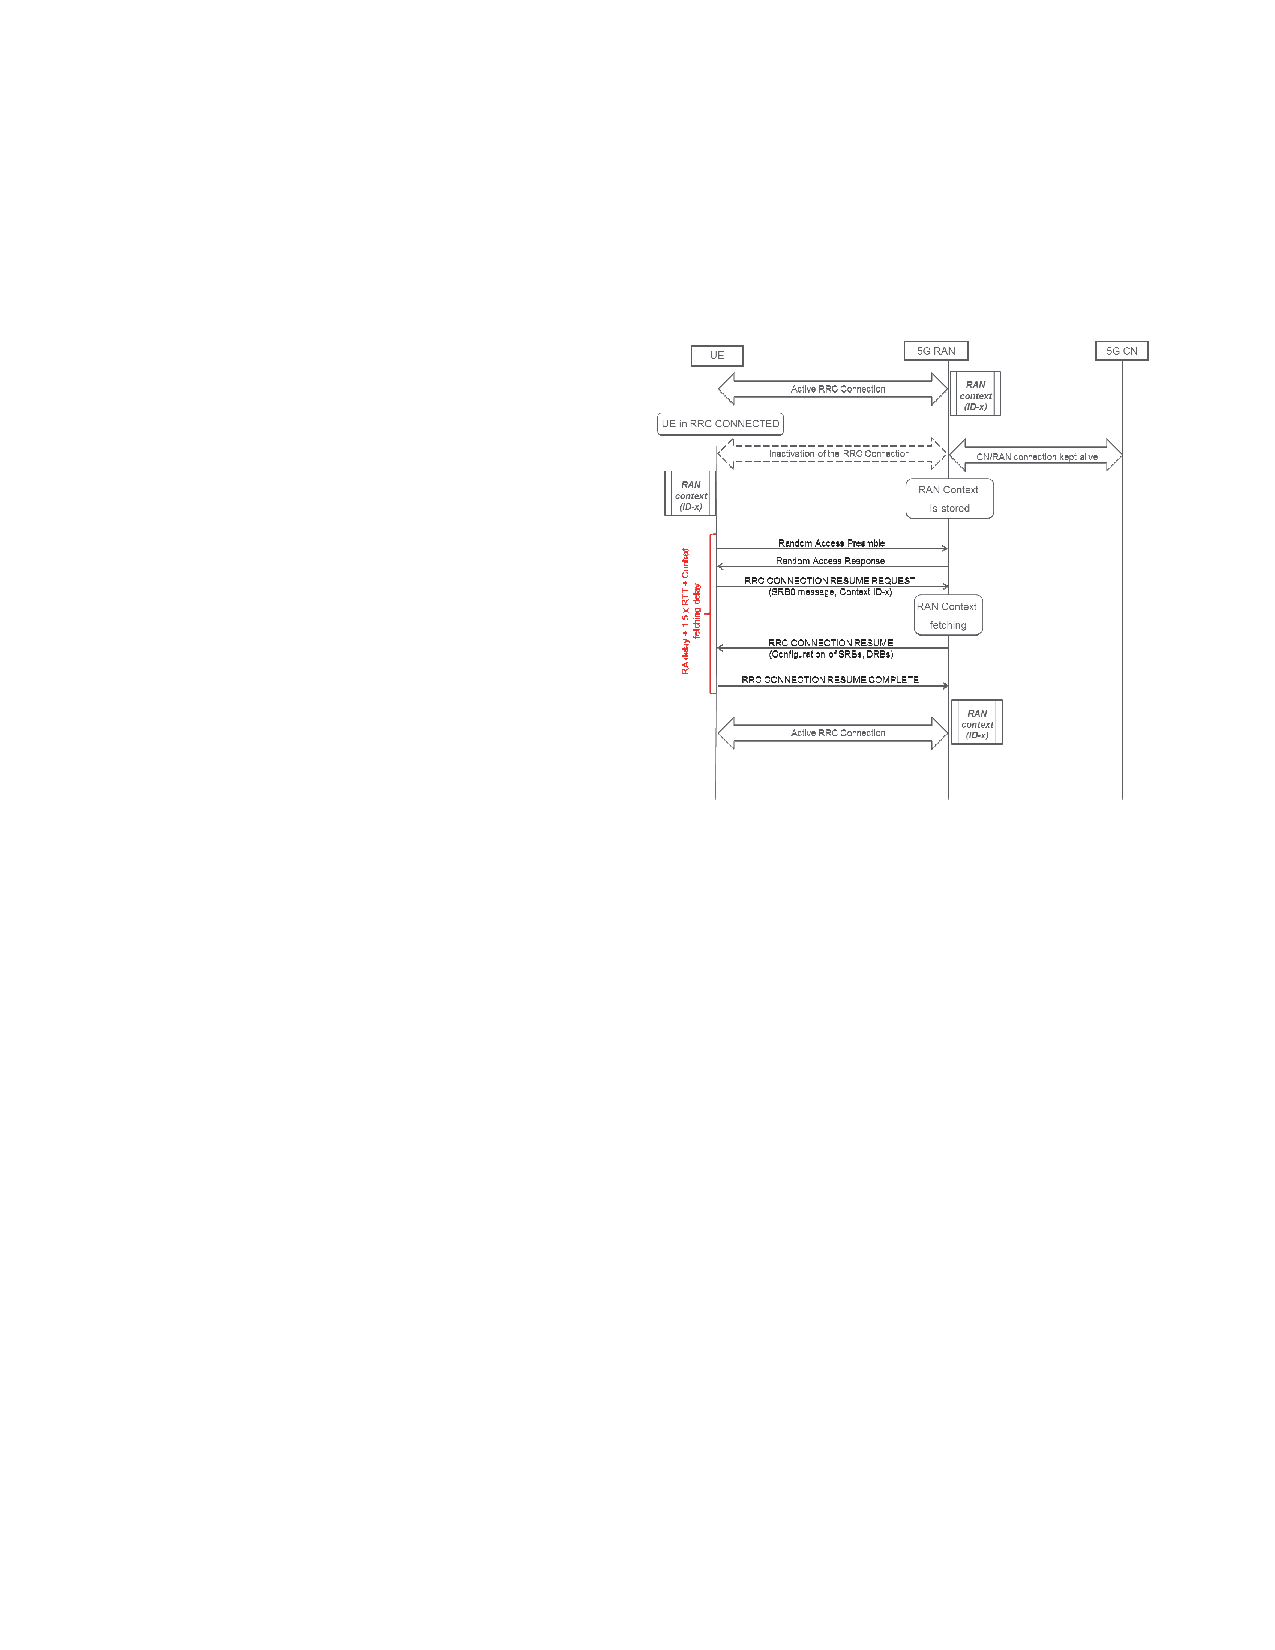
\includegraphics[width=0.9\hsize]{Signaling_for_the_RRC_CONNECTED_INACTIVE_to_RRC_CONNECTED_transition_for_the_novel_state_model.pdf}
%   \caption{Signaling for the RRC CONNECTED INACTIVE to RRC CONNECTED transition for the novel state model}
%   \label{Signaling_for_the_RRC_CONNECTED_INACTIVE_to_RRC_CONNECTED_transition_for_the_novel_state_model}
% \end{figure}

\clearpage
\subsection{シグナリング数のまとめ}
先行研究を調査することにより、状態遷移に伴うシグナリングの発生数が一部であるが、明らかになった。
図\ref{state_id}に示す状態遷移図と共に、状態遷移に伴って発生するシグナリングに関する情報を表\ref{table:signalings_all}に示す。

\begin{figure}[htbp]
  \centering
  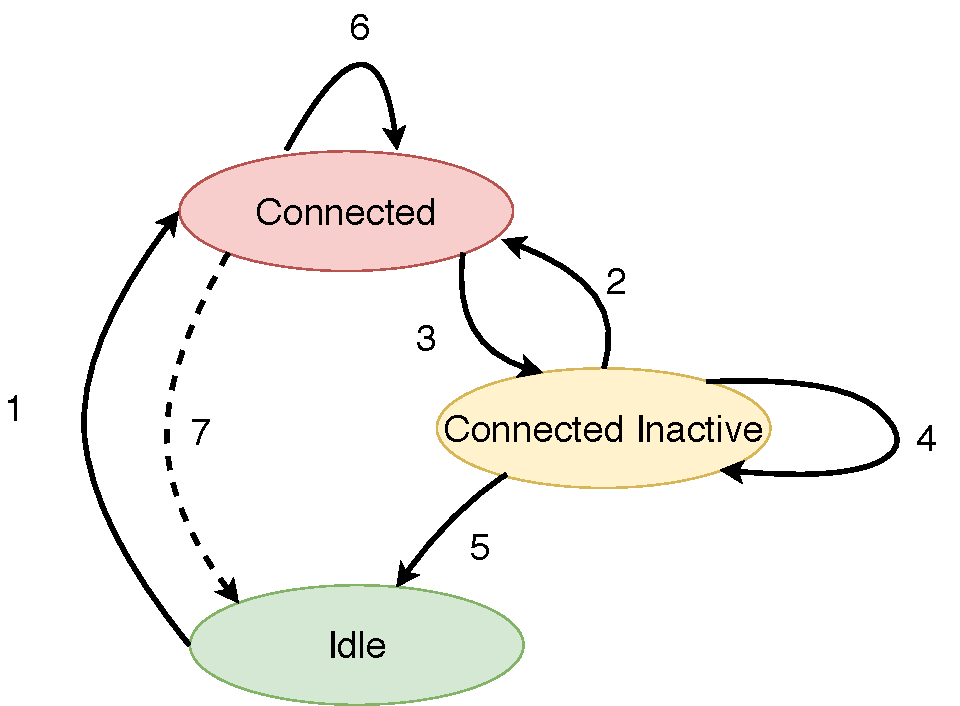
\includegraphics[width=0.9\hsize]{state_id.pdf}
  \caption{state transition}
  \label{state_id}
\end{figure}

\begin{table}[htbp]
  \centering
  \caption{Signaling Load}
  \label{table:signalings_all}
  \begin{tabular}{c|cccc|l}
    \hline
    遷移ID  & \multicolumn{4}{|c|}{シグナリング処理数} & 遷移条件                          \\
            & UE      & RAN     & MME     & SGW      &                                   \\ \hline \hline
    1       & 9       & 12      & 5       & 2        & Packets transmission              \\
    2       & 5       & 5       & 0       & 0        & 2 or more packets transmission    \\
    3       & 1       & 1       & 0       & 0        & Connected timer expiration        \\
    4       & 4       & 4       & 0       & 0        & One packet transmission           \\
    5       & 0       & 3       & 5       & 2        & Connected Inactive timer expiration             \\
    6       & 0       & 0       & 0       & 0        & Packets transmission              \\
    7       & 1       & 4       & 5       & 2        & Connected timer expiration            \\ \hline
  \end{tabular}
\end{table}


\section{今後の課題}
  \begin{itemize}
    \item 状態遷移に伴って発生するシグナリングの調査
    \item Connected Inactive状態において``状態遷移を伴わないデータ送信"が可能なデータ量の調査。
  \end{itemize}

\section*{\addcontentsline{toc}{section}{参考文献}}
\bibliographystyle{IEEEtran}
\bibliography{/Users/t-adachi/Documents/study/Bibliography/bib/hpt_core_network/myBib/LABbiblio,/Users/t-adachi/Documents/study/Bibliography/bib/hpt_core_network/Study_Group_Bibtex/bib/hptCoreNetwork_Study}
\end{document}
